
% ----------------------------------------------------------------------
%                   LATEX TEMPLATE FOR PhD THESIS
% ----------------------------------------------------------------------

% based on Harish Bhanderi's PhD/MPhil template, then Uni Cambridge
% http://www-h.eng.cam.ac.uk/help/tpl/textprocessing/ThesisStyle/
% corrected and extended in 2007 by Jakob Suckale, then MPI-CBG PhD programme
% and made available through OpenWetWare.org - the free biology wiki


%: Style file for Latex
% Most style definitions are in the external file PhDthesisPSnPDF.
% In this template package, it can be found in ./Latex/Classes/
\documentclass[oneside,a4paper,12pt]{Latex/Classes/PhDthesisPSnPDF}
\usepackage[utf8]{inputenc} %sisendfaili koodilehekylg UTF-8
\usepackage[T1]{fontenc} %täpitäht ühe sümbolina
\usepackage{enumerate}
\usepackage{graphicx}
\usepackage{float}
\usepackage{listings}
\usepackage{tikz}
\usetikzlibrary{arrows}
%\usepackage{indentfirst} %esimene lõik taandega
%: Macro file for Latex
% Macros help you summarise frequently repeated Latex commands.
% Here, they are placed in an external file /Latex/Macros/MacroFile1.tex
% An macro that you may use frequently is the figuremacro (see introduction.tex)
\include{Latex/Macros/MacroFile1}

\DeclareUnicodeCharacter{00A0}{ }

% ----------------------------------------------------------------------
       
% turn of those nasty overfull and underfull hboxes
\hbadness=10000
\hfuzz=50pt

%: --------------------------------------------------------------
%:                  NEW COMMANDS: definitions
% --------------------------------------------------------------

\newcommand{\HRule}{\rule{\linewidth}{0.5mm}}

%: --------------------------------------------------------------
%:                  FRONT MATTER: dedications, abstract,..
% --------------------------------------------------------------

\begin{document}


\lstset{basicstyle=\footnotesize\ttfamily}


%\language{english}

% sets line spacing
\renewcommand\baselinestretch{1.2}
\renewcommand{\chaptername}{}
\baselineskip=18pt plus1pt

%: ----------------------- generate cover page ------------------------

%\maketitle  % command to print the title page with above variables


%: ----------------------- cover page back side ------------------------
% Your research institution may require reviewer names, etc.
% This cover back side is required by Dresden Med Fac; uncomment if needed.

%\newpage
%\vspace{10mm}
%1. Reviewer: Name

%\vspace{10mm}
%2. Reviewer: 

%\vspace{20mm}
%Day of the defense:

%\vspace{20mm}
%\hspace{70mm}Signature from head of PhD committee:


%: ----------------------- Here comes the UT first page ------------------------
\begin{titlepage}

\begin{center}



\textsc{UNIVERSITY OF TARTU}\\

\textsc{FACULTY OF MATHEMATICS AND COMPUTER SCIENCE}\\

\texttt{Institute of Computer Science}\\[5cm]

% Title
%\HRule \\[0.4cm]
\textsc{ \large Lauris Kruusamäe}\\[0.5cm]
{\Huge \bfseries Energy-aware Sensor Data Collection for Mobile Users}\\[0.5cm]
{\large Bachelor Thesis (6 EAP)}\\[3cm]


%\HRule \\[1.5cm]

% Author and supervisor
%\begin{minipage}{0.4\textwidth}
%\begin{flushleft} \large
%\emph{Author:}\\
%John \textsc{Smith}
%\end{flushleft}
%\end{minipage}
\begin{minipage}{0.8\textwidth}
\begin{flushright} \large
\emph{Supervisor: Satish Narayana Srirama, PhD}  \\	  %degree (e.g. Phd, Msc, etc.)
\emph{Co-supervisor: Huber Flores, MSc}  %if any... and so on if more than 1
 %\textsc{Brown}
\end{flushright}
\end{minipage}

\textbf{}\\[1.0cm]

\textbf{Author:.................................... "....." May   2013}\\[0.5cm]

\textbf{Supervisor:............................... "....." May   2013}\\[0.5cm]

\textbf{Professor:................................. "....." May   2013}\\[0.5cm]        

\vfill
% Bottom of the page
{\large TARTU, 2013}

\end{center}

\end{titlepage}


%: ----------------------- abstract ------------------------

% Your institution may have specific regulations if you need an abstract and where it is to be placed in the document. The default here is just after title.


% Thesis Abstract -----------------------------------------------------


%\begin{abstractslong}    %uncommenting this line, gives a different abstract heading
\begin{abstracts}        %this creates the heading for the abstract page

Nowadays, mobile applications are becoming more context aware due to technological
achievements which enable the applications to anticipate users’ intentions. This is
achieved through using the device’s own micromechanical artifacts that can be used to
perceive the environment. However, this is constrained to the hardware limitations of
devices as not all devices provide the same options. Moreover, perceiving the environment strains the battery and therefore has its impact on devices' everyday usage.

To remedy this, a proposed solution has been made in the thesis “Context Sensor Data on
Demand for Mobile Users Supported by XMPP” by Kaarel Hanson. The solution is to gather the environmental data by specialized sensor modules and store it in a data server. Afterwards, devices can query the data from the server and thus gain access to information beyond the capabilities of their own hardware.

The solution uses XMPP for transporting sensor data from Arduino microcontrollers (sensor modules) to the cloud. Arduino provides low-cost hardware, while the cloud offers the reliable and high-
availability means for storing and processing sensor data. However, the developed prototype shows that running on a 9V battery the microcontroller lasts for 101
minutes when using an Ethernet module for communications, and 161,5 minutes with a
WiFi module. These results are not good enough for remote data collection with limited access as the maintenance cost would be too high when the batteries need to be replaced frequently. 

This thesis proposes an optimisation for the system so that instead of reading and
sending sensor data every 10 seconds, the cloud server would notify the controller
when to start sending data and when to stop. This means implementing an algorithm
for detecting similar sensor data readings and notifying the microcontroller of needed
operations. With similar readings, the microcontroller could be put to an idle state for
limiting power consumption, which would prolong battery life.

The aim is to optimise the sensor reading process enough to prolong the Arduino
microcontroller’s battery life on a 9V battery.

\end{abstracts}
%\end{abstractlongs}


% ---------------------------------------------------------------------- 


% The original template provides and abstractseparate environment, if your institution requires them to be separate. I think it's easier to print the abstract from the complete thesis by restricting printing to the relevant page.
% \begin{abstractseparate}
%   
% Thesis Abstract -----------------------------------------------------


%\begin{abstractslong}    %uncommenting this line, gives a different abstract heading
\begin{abstracts}        %this creates the heading for the abstract page

Nowadays, mobile applications are becoming more context aware due to technological
achievements which enable the applications to anticipate users’ intentions. This is
achieved through using the device’s own micromechanical artifacts that can be used to
perceive the environment. However, this is constrained to the hardware limitations of
devices as not all devices provide the same options. Moreover, perceiving the environment strains the battery and therefore has its impact on devices' everyday usage.

To remedy this, a proposed solution has been made in the thesis “Context Sensor Data on
Demand for Mobile Users Supported by XMPP” by Kaarel Hanson. The solution is to gather the environmental data by specialized sensor modules and store it in a data server. Afterwards, devices can query the data from the server and thus gain access to information beyond the capabilities of their own hardware.

The solution uses XMPP for transporting sensor data from Arduino microcontrollers (sensor modules) to the cloud. Arduino provides low-cost hardware, while the cloud offers the reliable and high-
availability means for storing and processing sensor data. However, the developed prototype shows that running on a 9V battery the microcontroller lasts for 101
minutes when using an Ethernet module for communications, and 161,5 minutes with a
WiFi module. These results are not good enough for remote data collection with limited access as the maintenance cost would be too high when the batteries need to be replaced frequently. 

This thesis proposes an optimisation for the system so that instead of reading and
sending sensor data every 10 seconds, the cloud server would notify the controller
when to start sending data and when to stop. This means implementing an algorithm
for detecting similar sensor data readings and notifying the microcontroller of needed
operations. With similar readings, the microcontroller could be put to an idle state for
limiting power consumption, which would prolong battery life.

The aim is to optimise the sensor reading process enough to prolong the Arduino
microcontroller’s battery life on a 9V battery.

\end{abstracts}
%\end{abstractlongs}


% ---------------------------------------------------------------------- 

% \end{abstractseparate}

%: ----------------------- tie in front matter ------------------------

%\frontmatter
%\include{0_frontmatter/dedication}
%\include{0_frontmatter/acknowledgement}


%: ----------------------- contents ------------------------

\setcounter{secnumdepth}{3} % organisational level that receives a numbers
\setcounter{tocdepth}{3}    % print table of contents for level 3
\tableofcontents            % print the table of contents
% levels are: 0 - chapter, 1 - section, 2 - subsection, 3 - subsection


%: ----------------------- list of figures/tables ------------------------
\newpage
\listoffigures	% print list of figures
\newpage
\listoftables  % print list of tables


%: ----------------------- glossary ------------------------

% Tie in external source file for definitions: /0_frontmatter/glossary.tex
% Glossary entries can also be defined in the main text. See glossary.tex
%\include{0_frontmatter/glossary} 

%\begin{multicols}{2} % \begin{multicols}{#columns}[header text][space]
%\begin{footnotesize} % scriptsize(7) < footnotesize(8) < small (9) < normal (10)

%\printnomenclature[1.5cm] % [] = distance between entry and description
%\label{nom} % target name for links to glossary

%\end{footnotesize}
%\end{multicols}

%%%%%%%%%%%%%%%%%%%%%%%%%%%%%%%%%%%INCLUDE LATEX SUBDOCUMENTS%%%%%%%%%%%%%%%%%%%%%%%%%%%%%%%%%%%%%%%%%%%%

%: --------------------------------------------------------------
%:                  MAIN DOCUMENT SECTION
% --------------------------------------------------------------

% the main text starts here with the introduction, 1st chapter,...
\mainmatter

%: ----------------------- subdocuments ------------------------

% Parts of the thesis are included below. Rename the files as required.
% But take care that the paths match. You can also change the order of appearance by moving the include commands.

%\include{0_frontmatter/acknowledgement} % optional

% this file is called up by thesis.tex
% content in this file will be fed into the main document

%: ----------------------- introduction file header -----------------------

\chapter{Introduction}

% the code below specifies where the figures are stored
\ifpdf
    \graphicspath{{1_introduction/figures/PNG/}{1_introduction/figures/PDF/}{1_introduction/figures/}}
\else
    \graphicspath{{1_introduction/figures/EPS/}{1_introduction/figures/}}
\fi

% ----------------------------------------------------------------------
%: ----------------------- introduction content -----------------------
% ----------------------------------------------------------------------



%: ----------------------- HELP: latex document organisation
% the commands below help you to subdivide and organise your thesis
%    \chapter{}       = level 1, top level
%    \section{}       = level 2
%    \subsection{}    = level 3
%    \subsubsection{} = level 4
% note that everything after the percentage sign is hidden from output



\section{Introduction} % section headings are printed smaller than chapter names

Mobile applications are becoming more context aware and depend on perceiving the surrounding environment to provide users with the best functionality possible. This is achieved due to technological advances that enable the device to sense the surroundings, however, these abilities are limited to each device's hardware configuration.

A proposed solution has been made in the thesis "Context Sensor Data on Demand for Mobile Users Supported by XMPP" by Kaarel Hanson \cite{prev_thesis}. The solution is to have special sensor modules perceive the environment and gather the measurements in a central data center, which can then be used to provide data to mobile users. 

A prototype was developed based on Arduino for the sensors and XMPP for communication. This thesis proposes improvements to the existing prototype to enable sleep mode for the sensor modules and data prediction on the data server side. These improvements help prolong battery life on a 9V battery, which was measured to be 161,5 minutes with the existing prototype. 

Without enough battery life, the overhead of using the modules to gather data makes the solution inefficient. Therefore, it is crucial to make the modules last longer, which is the main goal of this thesis.

\subsection{Motivation}
The developed prototype \cite{prev_thesis} works well when the general idea and goal is considered. However, the lack of flexibility of data transmission intervals and high power needs constrain the implementation usages. In order to take full advantage of the prototype, power usage should be reduced and more flexibility added to the communication between the server-side client and sensor modules.  

\subsection{Contributions}

A more flexible data collection solution is developed based on HTTP. The changes made enable more energy-efficient data collection by predicting sensor data when possible. A fuzzy control system was developed to decide if sensor data is predictable and for what time period.  Moreover, the prototype's Arduino-based sensor module has been improved to support sleep mode while no sensor data is sent to the server-side client. Power consumption before and after the changes was tested to indicate changes' effect on battery life. 

\subsection{Outline}

%for example
%\noindent \textbf{Chapter 2}: discusses the state of the art addressed by this thesis. 

\noindent \textbf{Chapter 2}: introduces the Arduino framework and modules used in the prototype. Finally, a description of fuzzy control systems and simple linear regression is given.
\newline

\noindent \textbf{Chapter 3}: describes the existing prototype and gives an overview of its implementation details. Later, an overview of identified areas of improvement is given.
\newline

\noindent \textbf{Chapter 4}: explains the improvements made to the prototype. Firstly, describes changes made to the Arduino sensor module. Secondly, changes in the communication between the sensor module and the server-side client are discussed. Lastly, an overview of the server-side fuzzy control system and data prediction techniques is given. The chapter is ended by a power consumption comparison between the initial and improved prototype.
\newline

\noindent \textbf{Chapter 5}: draws conclusions and summarizes the results.
\newline

\noindent \textbf{Chapter 6}: discusses a related paper and the thesis on which the current work is based on.
\newline

\noindent \textbf{Chapter 7}: points out some areas of the prototype which can be developed further to improve the results.
\newline

%\noindent \textbf{Chapter 3}: explains the problems regarding the combination and the invocation of cloud services from the mobile phone. 



	% background information
% this file is called up by thesis.tex
% content in this file will be fed into the main document

\chapter{State of the Art} % top level followed by section, subsection


%transition between chapters, usually no more than two parragraphs
The state of the art used in the thesis highlighted the advances in the cloud computing domain and the mobile domain...


% change according to folder and file names
\ifpdf
    \graphicspath{{X/figures/PNG/}{X/figures/PDF/}{X/figures/}}
\else
    \graphicspath{{X/figures/EPS/}{X/figures/}}
\fi

% ----------------------- State of the art ------------------------
%We will try to target 20 -25 word pages for this work
%probably after changing to Latex, the amount of pages will increase but that's because the template
%is double space and half page of each chapter is lost at the beginning, among others.

%XMPP description should fit in one page
\section{Jabber and XMPP}
Description of Jabber and XMPP protocol and its usage.

%arduino along with its component should be one and half page
%if there are configuration we will put them in the appendix
%or we can put a footnote with a link to your github account
\section{Arduino}
Introduction to Arduino.

\subsection{Arduino Mega ADK}
Overview of the Arduino Mega ADK board and its components.

\subsection{TinkerKit}
Overview of the TinkerKit module, components and sensors.

\subsection{Modules}
Overview of the Ethernet and Wireless Shields and WiFly wireless module.

%Fuzzy logic is the main contribution, therefore, you can write here up to 5 pages
\section{Fuzzy Logic}
Description of fuzzy logic and its uses.

%This one is not necessary, since we will just mention the tool and it will be cited in chapter 4
%\section{Power supply}
%Overview of the PeakTech 1890 power supply.

%Instead, try to investigate about related works
%both from academic and commercial points of view, it is unlikely that there is a commercial tool about it, but 
%maybe there is something, you can look for solutions for monitoring smart environments or so
%try to target 2 pages max. One or two paragraphs describing each solution
\section{Related Works}
%Some academic related work that can be mentioned is described below
%try to look for them in Google scholar
%From Instant Messaging to Cloud computing, a XMPP review (paper)
%XMPP for cloud computing in bioinformatics supporting discovery and invocation of asynchronous web services
%Performance Evaluation of XMPP on the Web

%

%add figures
%\begin{figure}
%\centering
%\includegraphics[width=0.65\textwidth]{2/figures/Cloud/funambolArchitecture.png}
%\caption{Funambol architecture}
%\label{fig:funambolArchitecture}
%\end{figure}


% ---------------------------------------------------------------------------
% ----------------------- end of thesis sub-document ------------------------
% --------------------------------------------------------------------------- 
	        	% state of the art
% this file is called up by thesis.tex
% content in this file will be fed into the main document

%: ----------------------- name of chapter  -------------------------
\chapter{Problem Statement} % top level followed by section, subsection

%: ----------------------- paths to graphics ------------------------

% change according to folder and file names
\ifpdf
    \graphicspath{{X/figures/PNG/}{X/figures/PDF/}{X/figures/}}
\else
    \graphicspath{{X/figures/EPS/}{X/figures/}}
\fi

%: ----------------------- Mobile Cloud Middleware ------------------------

In this chapter, the prototype developed in Context Sensor Data on Demand
for Mobile Users Supported by XMPP \cite{prev_thesis} is described. The prototype was successful, but had some downsides. Secondly, an overview of the problems with the existing implementation is given. 
\todo{Add a small introduction of who wrote the previous thesis etc}

\section{Current Solution}

The current solution \cite{prev_thesis} has three main components:
\begin{enumerate}
\item Arduino sensor module
\item OpenFire XMPP server
\item Data collection server in the cloud (referred to as the server from here on)
\end{enumerate}

There were two separate configurations described in Context Sensor Data on Demand
for Mobile Users Supported by XMPP - one using Wi-Fi and the other Ethernet for network communication. Only Wi-Fi configuration is considered in this thesis due to the fact that the availability of an Ethernet connection (a cable) usually means that there is a power outlet nearby. 

\subsection{Arduino}

The first component is the Arduino sensor module. The hardware configuration is based on the Arduino Mega ADK board. Wireless Shield with RN-XV WiFly module is mounted on top of the board. Wireless Shield and Arduino board communicate over UART (hardware serial). TinkerKit Mega Sensor Shield is mounted on top of the Wireless Shield with 7 modules attached to it: 4 LED indicator lights, Hall, thermistor and LDR sensors. The external power source used is a 9V battery.

On the software side, the implementation mainly relies on a XMPP library and WiFly module library called WiFlyHQ. The WiFlyHQ library is responsible for creating a TCP connection and communication over the network, the XMPP library handles all the XMPP implementation details. 

The sketch itself is fairly straightforward - in $setup()$ a wireless network is joined, a TCP connection established and lastly a XMPP session is initialized. In $loop()$ all connections are checked and reestablished if needed. Then the last transmit time variable is compared to the current time and if the report step amount (currently 10 seconds) has passed, data is collected from the sensors, formatted to appropriate JSON string and sent to the server-side client. 

\subsection{XMPP Communication}

Both the data collection server and Arduino module are XMPP clients. The XMPP OpenFire server runs in the cloud and provides XMPP communications to both clients. Clients connect to the same chat where the server listens for messages from the sensor module. When a message is received by the server, sensor data is parsed from it and saved in a database.

\todo{xmpp initialization time}
XMPP session lifecycle can be seen in \autoref{xmpp_lifecycle}. With the current implementation, steps 1 - 5 are done once when establishing the connection or when the connection drops. Data transmission step is done every 10 seconds and the last 2 steps are done when the connection is closed.

\begin{figure}[H]
\label{xmpp_lifecycle}
\centering
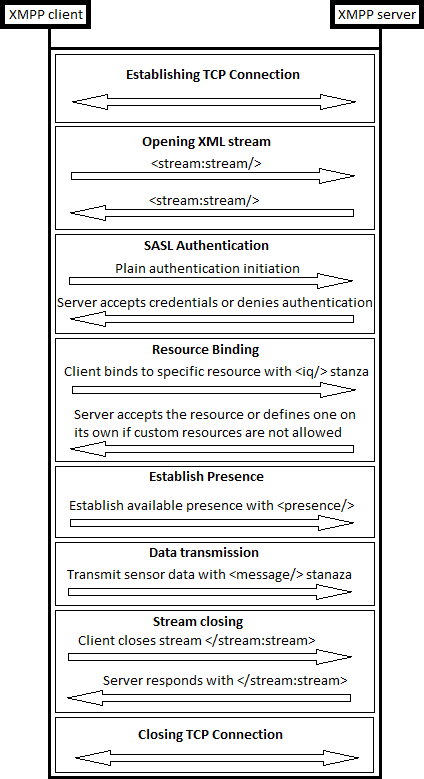
\includegraphics[scale=0.6]{3/figures/xmpp_session.png}
\caption{XMPP Session Lifecycle}
\end{figure}

\subsection{Data Collection Server}
The data collection server is responsible for gathering sensor data and saving it in a database. Its implementation is written in Java and uses Smack XMPP API to communicate over XMPP. Data is stored in a H2 database, because of its simplicity and suitability for prototyping. 

The database has three main tables - sensors, data and locations. Locations table has different sensor module locations, sensors table has different types of sensors and data has data gathered from different locations and sensors. The data model can be seen in \autoref{data_model_initial}.

\begin{figure}[H]
\label{data_model_initial}
\centering
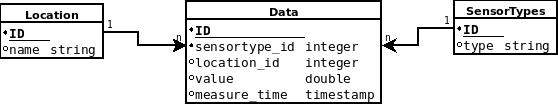
\includegraphics[scale=0.6]{3/figures/data_model_initial.jpg}
\caption{Server-side Data Model}
\end{figure}

\section{Problems}

Previously mentioned implementation has a few problems which will be discussed in this section. The two main points are power consumption and data collection flexibility. 

According to the tests run in the previous thesis, the battery is able to power the module for 161,5 minutes using Wi-Fi. \cite[p. 50-51]{prev_thesis} This, however, is not sufficient to enable actual data collection from a remote location. The problem can be addressed by using a larger battery, but the actual power consumption should be optimized, too. Additionally, the 10 second data transmission interval is hard coded into the Arduino sensor module, which does not provide enough flexibility. The following chapter described changes to the hardware, software and communication methods which improve on these error points.

\subsection{Hardware}

The hardware configuration has two main problems. Firstly, communication over the wireless module can be unstable at times, because parts of the messages might be missing or scrambled when read from the UART \cite[p. 47]{prev_thesis}. Since XMPP session initialization is quite verbose, the possibility of receiving scrambled or incomplete messages effects the process. 

Secondly, all parts of the hardware configuration are run in full power mode. As there is a 10 second gap between data transmission and sensor reads, there is a time period when most components are idling. This, in turn, means that some parts of hardware could use less power during these intervals and therefore reduce overall power consumption.

\subsection{Software}

With the existing implementation $loop()$ is called consecutively and time differences are checked to determine when 10 seconds has passed using the internal $millis()$ function, which gives the current Unix time. Since we have a 10 second interval, we do not need to waste cycles on time difference checks we now will fail for the next 10 seconds. A way to delay program execution could be used to stop the execution until we know the defined amount of time has passed. 

In addition, as messages from the Wireless Shield might not be complete and  XMPP session initialization is a verbose process, the current XMPP implementation hangs when scrambled messages are received during session start up. The library checks from complete XML tags, but when the attributes are incomplete, connection will not be successful and the session initialization code hangs.

\subsection{Power Consumption}

Power consumption is the main problem this thesis focuses on. As a 9V battery has an average capacity of 400 $mAh$ at 100 $mA$ current, the resource is quite limited. With the existing configuration, the average current drawn is 108 $mA$. Battery lifetime tests in the previous thesis showed that the module runs for 161,5 minutes on a 9V battery \cite[p. 50]{prev_thesis}. However, 161,5 minutes is not enough to gather contextual data for the proposed data collection system. The batteries need to be changed too often for it to be a viable solution. 
\todo{how should i reference all the data collected?}


% ---------------------------------------------------------------------------
%: ----------------------- end of thesis sub-document ------------------------
% ---------------------------------------------------------------------------

		% problem statement
% this file is called up by thesis.tex
% content in this file will be fed into the main document

%: ----------------------- name of chapter  -------------------------
\chapter{Problem Solution} % top level followed by section, subsection

In this chapter improvements to the existing implementation are discussed. First, changes in the Arduino sensor module are described. Secondly, an overview of changes in the communication between the module and data collection server (the server from here on). Lastly, an overview of the fuzzy control and data prediction systems that were implemented to reduce communication overhead and power consumption.

The main goal is to reduce the average power consumption measured by \todo{reference it somehow} the PeakTech power supply. 

\todo{introduction}

%: ----------------------- paths to graphics ------------------------

% change according to folder and file names
\ifpdf
    \graphicspath{{X/figures/PNG/}{X/figures/PDF/}{X/figures/}}
\else
    \graphicspath{{X/figures/EPS/}{X/figures/}}
\fi

\section{Power Consumption}

The first problem addressed is power consumption. There are two main ideas behind reducing it - put the sensor module to sleep mode when not transmitting data and reduce the need for data transmission. For this, the server-side client was improved to predict sensor data when possible and notify the sensor module of the next data transmission time. This enables the module to enter sleep mode for the given time period and thus reduce power consumption. 

\subsection{Sleep}

Since the module consists of 3 components - Arduino Mega ADK, Wireless SD Shield with WiFly module and TinkerKit Sensor Shield. Both the Mega ADK and WiFly module support sleep modes. 

\subsubsection{Watchdog Timer}
A watchdog timer \cite{watchdog_timer} is an electronic timer used to recover from computer malfunctions. They are found in automated systems where human interference is not possible and therefore the system must be able to recover from malfunctions on its own. 
A watchdog timer essentially performs a timing function producing a delayed response to an input trigger. The most common implementation has a digital counter that counts from a specified value down to a terminal value. Usually the initial value is programmable. When the counter reaches the terminal value, the timer timeouts and triggers a timeout signal. Usually this means restarting the program from the start. A program can restart the watchdog timer at any time. The act of restarting is usually referred to as "kicking the dog". In this way, a program can be written witch never lets the counter reach the terminal value.

\subsubsection{Arduino Mega ADK}

In case of an Arduino board, when the watchdog timer timeouts, the sketch is restarted (new call to $setup()$). Furthermore, a watchdog timeout signal is sent and this signal can be captured by the sketch. In the Arduino sketch, this is implemented by the JeeLib library \cite{jeelib_general}. JeeLib is a library written for experimenting with JeeLabs products, however, some parts of the library are written for Arduino boards and can be used with them. Specifically, the Ports class \cite{jeelib_port} is the one used in this implementation to put the Arduino Mega ADK into sleep mode. The sketch execution stops for the specified sleep time and afterwards execution continues from the call to sleep function.

\todo{Add a sample overview of the sketch here maybe?}

\subsubsection{WiFly module}

The RN-XV WiFly module can be put to sleep in two ways - sleep timer or sleep command. With the sleep timer, the shield will enter sleep mode after a specified time period has passed since all TCP active connections have closed. With the sleep command the module will enter sleep mode immediately, unless an active TCP connection exists. \cite{wifly_manual}. 

This means that in order to put the WiFly module to sleep, all active connections must be closed. For the XMPP session, this means closing the active stream and the underlying TCP connection. Once this has been done, the module can successfully enter sleep mode. 

The module can be waken up by either sending characters of the UART or by using the wake timer. In our implementation the activity on the UART wakes the module up when the sketch execution continues after the Mega ADK wakes up from sleep mode and establishes a new TCP connection in the start of $loop()$ method call. This effectively means going through the first 5 stages of XMPP session lifecycle on every wake up. 
Since XMPP session initialization is quite verbose and the communication over Wi-Fi is unstable, the possibility of receiving scrambled or incomplete messages creates a problem. 

\subsection{Communication}

Because all TCP connections and therefore the XMPP session have to be closed after every data transmit, XMPP session lifecycle steps 1 - 5 shown in \autoref{xmpp_lifecycle} are executed multiple times. When testing the XMPP implementation with Arduino Mega ADK and WiFly module sleep modes enabled, a troubling fact was discovered - the XMPP session negotiation fails at least once for every 30 minute test. The reason for these connection failures are scrambled authentication or stream opening stanzas. 

From the tests, it could be seen that the average XMPP session start up time was 15 seconds. \todo{show a graph here i guess? or whatever} Data needs to be transmitted every 10 seconds, which means that the module can never be put to sleep as it will not be able to go through the sleep and wake up cycle during the available time period. Moreover, data transmission took on average 1 second, meaning that 15 seconds spent on wake up would result in a second of actual work, which is not efficient. 

During testing the sleep and wake up cycles with XMPP, it was found that XMPP session negotiation will hang approximately once in 15 minutes. As the maximum sleep time in our implementation is 65 seconds, this means that there are at least 13 separate session negotiations. Of course, this is the problem of the XMPP library in use and its lack of error handling. Problems with the library could be addressed with a better implementation, however, there was another factor discovered during the tests.

As a result, XMPP as a means of communication was not viable when trying to minimize power consumption. As an alternative, \todo{look how to reference these} web sockets, raw sockets and HTTP was considered. Web sockets were left out because opening a web socket connection is opened with a HTTP request, making using that one request to actually send the data more efficient. Therefore, HTTP was preferred to web sockets. Raw socket implementation in Arduino would add needless complexity to the sketch and was therefore not implemented. 

The main advantages of HTTP are connection initialization speed and simplicity. The average time to wake up from sleep mode, send an HTTP request and receive response from the server, was measured to be around 6 seconds. In the previous scenario of 10 second transmission interval, it would mean 4 seconds could be spent in sleep mode, 4 seconds to wake up and transmit the data. This implementation would be more energy efficient, which can be seen in \autoref{30s_interval_power}. The data was gathered while running the prototype for 30 minutes with a data sending interval of 30 seconds. The sleep times were adjusted for both configurations based on their wake up times. As seen in the figure, the HTTP configuration consumes approximately 20\% less power than the one using XMPP. 

\todo{Add a sample request here}

\begin{figure}[h]
\centering
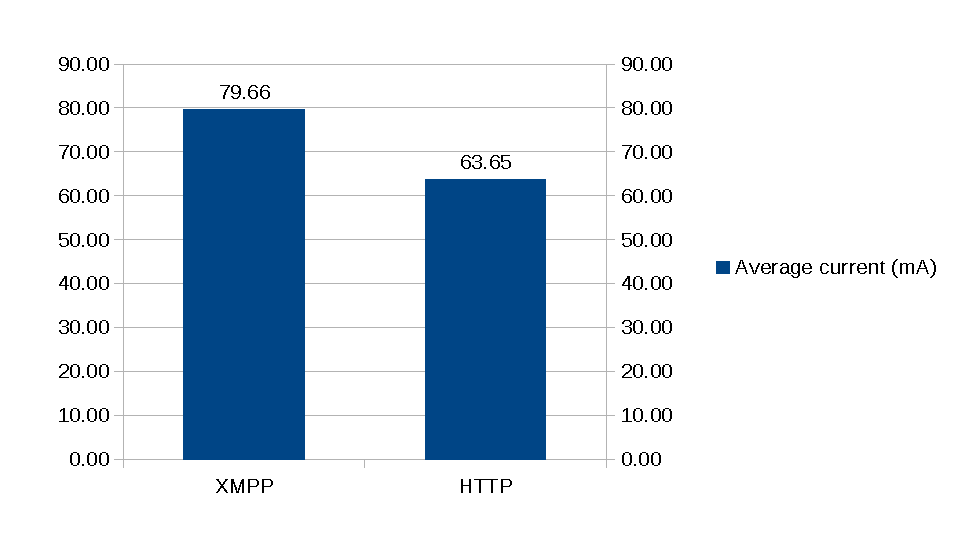
\includegraphics[scale=0.9]{4/figures/30s_xmpp_vs_http.pdf}
\caption{Power Consumption at 30 Second Interval}
\label{30s_interval_power}
\end{figure}

\section{Server-side Client}

With the move from XMPP to HTTP, the server-side client's implementation changed. Instead of using XMPP Smack library, a web server was needed. Jetty was selected because of its simplicity and possibility to embed it into the application. A web server embedded in an application is useful when prototyping, because it saves time on configuration and deployment. 

Furthermore, to take full advantage of the newly developed sleep mode functionality, the client was further developed to predict sensor values for some time. Two modules were added the server for this - simple linear regression and fuzzy control engine. In addition, the data model was modified to suit the new modules. The new data model can be seen in \autoref{data_model_final}. $Data$ table now has $measured$ field, which indicates if the value has been measured or predicted. $SensorTypes$ table has two new fields - $regression\_error$ and $measure\_error$. $regression\_error$ is the acceptable regression model error for future predictions. $measure\_error$ indicates the acceptable variance for measured values. 

\todo{Do i really need this here?}
The final web server consists of 4 modules:
\begin{enumerate}
\item Request handler
\item Linear regression model
\item Fuzzy control engine
\item Data storage
\end{enumerate}

\begin{figure}[h!]
\centering
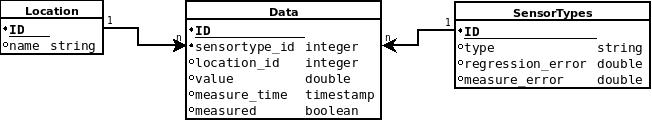
\includegraphics[scale=0.6]{4/figures/data_model_final.jpg}
\caption{Updated Server-side Data Model}
\label{data_model_final}
\end{figure}

\subsection{Simple Linear Regression}

A simple linear regression model was selected to predict future data, which uses the least squares method to calculate the future values. \todo{add a mention of the paper the idea was taken from?} The model has a single explanatory variable - Unix time. This variable is used to predict the future values of sensor readings based on previous measurements. 

The model sample is taken from previous measurements during the last 4 minutes. The 4 minute interval is selected to balance out errors caused by extreme values. This is necessary because a single value with big enough deviation can cause the regression model to become inaccurate. 

To measure the accuracy of the model, an confidence level of 90\% was introduced. If the sample for last 4 minutes provides an accurate enough regression model, then the predictions can be used. Otherwise, fresh data should be queried and added to the model until the error threshold is satisfied. The equation to calculate regression model's confidence level $\alpha$:\\

\begin{center}
$\alpha = 2\Phi \left ( \frac{\epsilon}{STDEV[e]}  \right ) - 1$.
\end{center}

Here $\Phi$ is the CDF (Cumulative Distribution Function) of residuals, $\epsilon$ is the allowed error (in the database model named as $regression\_error$ and $STDEV[e]$ is the standard deviation of residuals (also known as standard error of estimate). \todo{look this part over, should be ok}

Regression models are created separately for each sensor. Each model has a sample of previous measurements and the allowed error $\epsilon$ defined in the database. 
The confidence level $\alpha$ is calculated for each model and has to be over $90\%$ which is the selected confidence threshold. If all regression models satisfy the confidence level, then the fuzzy control system is initialized with data from previous measurements and calculated confidence levels. 

\subsection{Fuzzy Logic Engine}

The next step in predicting future sensor values is to calculate the time interval for the next measurement request. To calculate the time, a fuzzy control system was introduced to provide flexible decisions based on multiple input variables. The input variables are: 
\begin{enumerate}
\item $temp$					
\item $temp$ $predictability$	
\item $light$					
\item $light$ $predictability$	
\item $hall$					
\item $hall$ $predictability$
\end{enumerate}

Here each sensor has a pair of input variables - measured sensor value and sensor value predictability (regression model confidence level $\alpha$). All these variables are mapped into fuzzy sets, a procedure call fuzzification. The predictability variables are mapped into sets which all have the same membership functions shown in figure \autoref{pred_sets}.

\begin{figure}[h!]
\centering
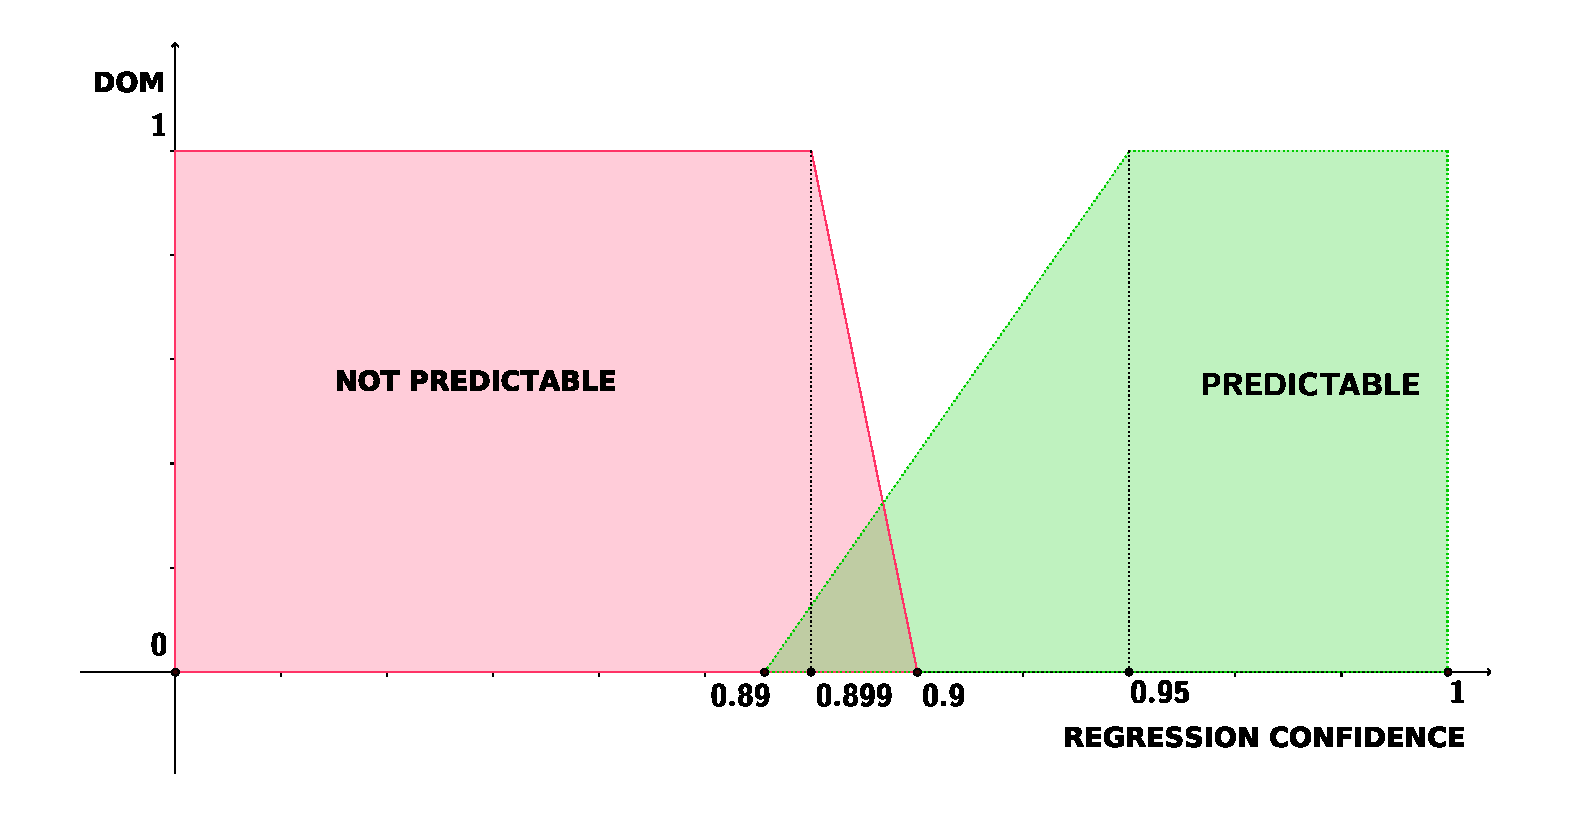
\includegraphics[scale=0.58]{4/figures/pred_sets.pdf}
\caption{Regression Confidence Fuzzy Sets}
\label{pred_sets}
\end{figure}

The fuzzy control system is initialized with a previous measurement for each sensor. This effectively sets the bounds of each sensor's fuzzy sets as seen in \autoref{change_sets}. The $PREDICTABLE$ fuzzy set's DOM (degree of membership) reaches maximum at a confidence level of 0.95 or 95\% because for our prototype anything above that level is highly predictable. 

The measured sensor values are fuzzified into sets, which each have different membership functions. The membership functions are calculated on the last measurement received as seen in \autoref{change_sets}. Here $X$ in set labels notes the sensor type currently used as the sets are the same relative to each sensor's previous measurement. The center point $O$ is the previously measured value. $||X_2X_3||$ is the predefined sensor measurement error  ($sensor\_error$ field in the data model). This means that if the new measurement is between the points $X_2$ and $X_3$, there is no change in the measurement for the fuzzy system. The lengths $||X_0X_2||$, $||X_1O||$, $||OX_4||$ and $||X_3X_5||$ are defined by the same variable $slope\_width$. Currently, slope width is the same as the selected $regression\_error$ values which are 5 times the value of $measure\_error$. The selected error values can be seen in \autoref{errors_table}. 

\begin{figure}[h!]
\centering
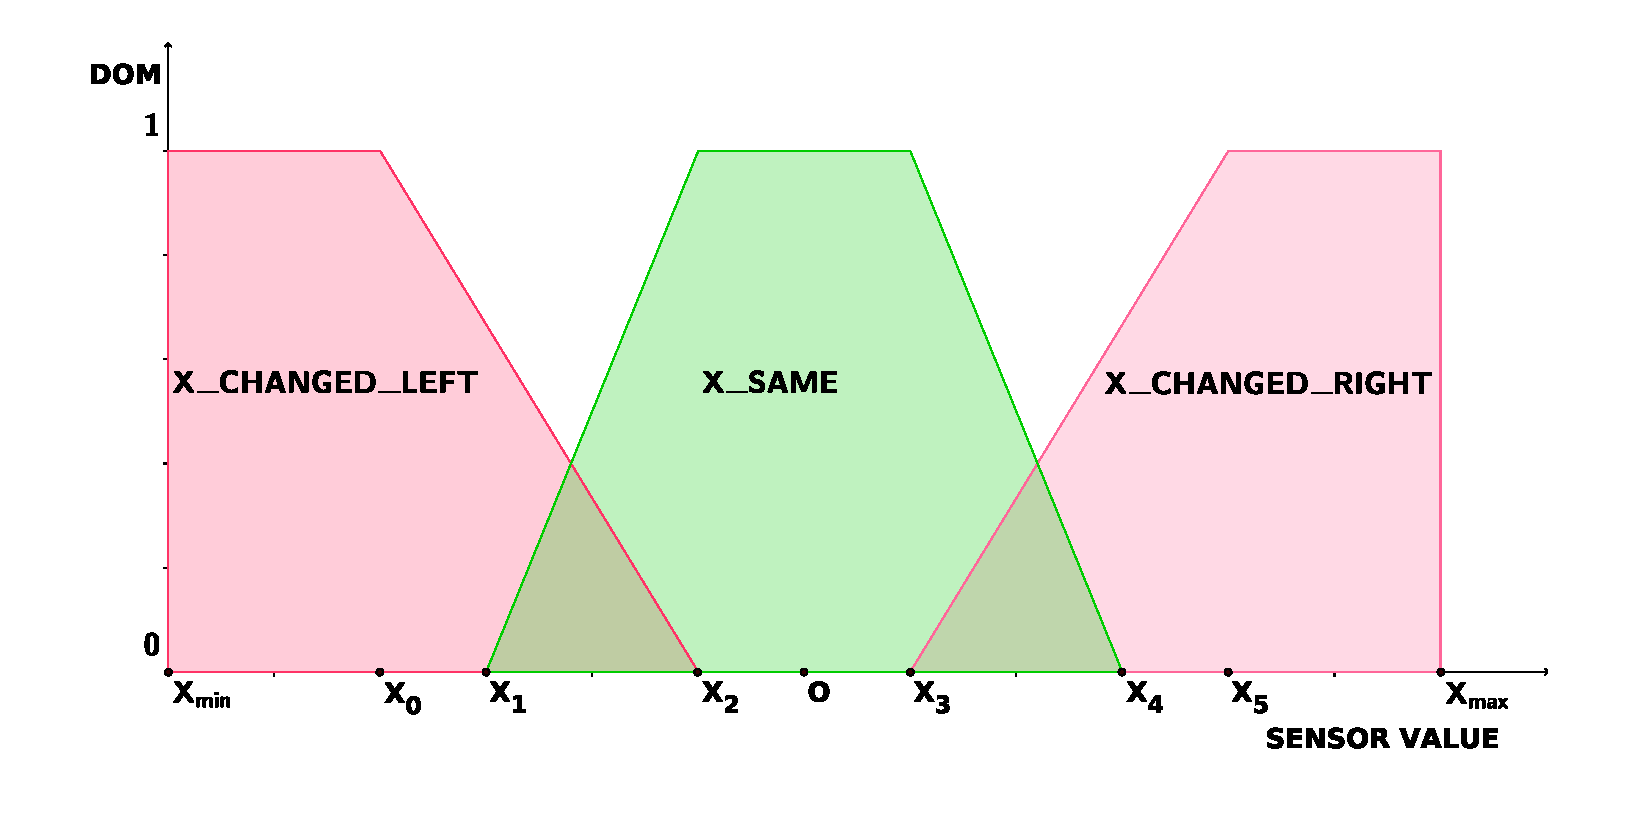
\includegraphics[scale=0.55]{4/figures/change_sets.pdf}
\caption{Sensor Value Fuzzy Sets}
\label{change_sets}
\end{figure}

\begin{table}[h]
\centering
  \begin{tabular}{| l | l | l | l |}
    \hline
     & Temp & Hall & LDR \\ \hline
    $measure\_error$ & 0.1 & 0.5 & 10 \\ \hline
    $regression\_error$ & 0.5 & 2.5 & 50 \\
    \hline
  \end{tabular}
\caption{Selected Error Values}
\label{errors_table}
\end{table}

The output variable is defuzzified from the idle time sets which have membership functions described in \autoref{idle_sets}. The sets $request$ and $predict$ are symmetrical to enable easy defuzzification. The maximum idle time is 65 seconds, which is the maximum length of one sleep cycle for the sensor module. 

\begin{figure}[h!]
\centering
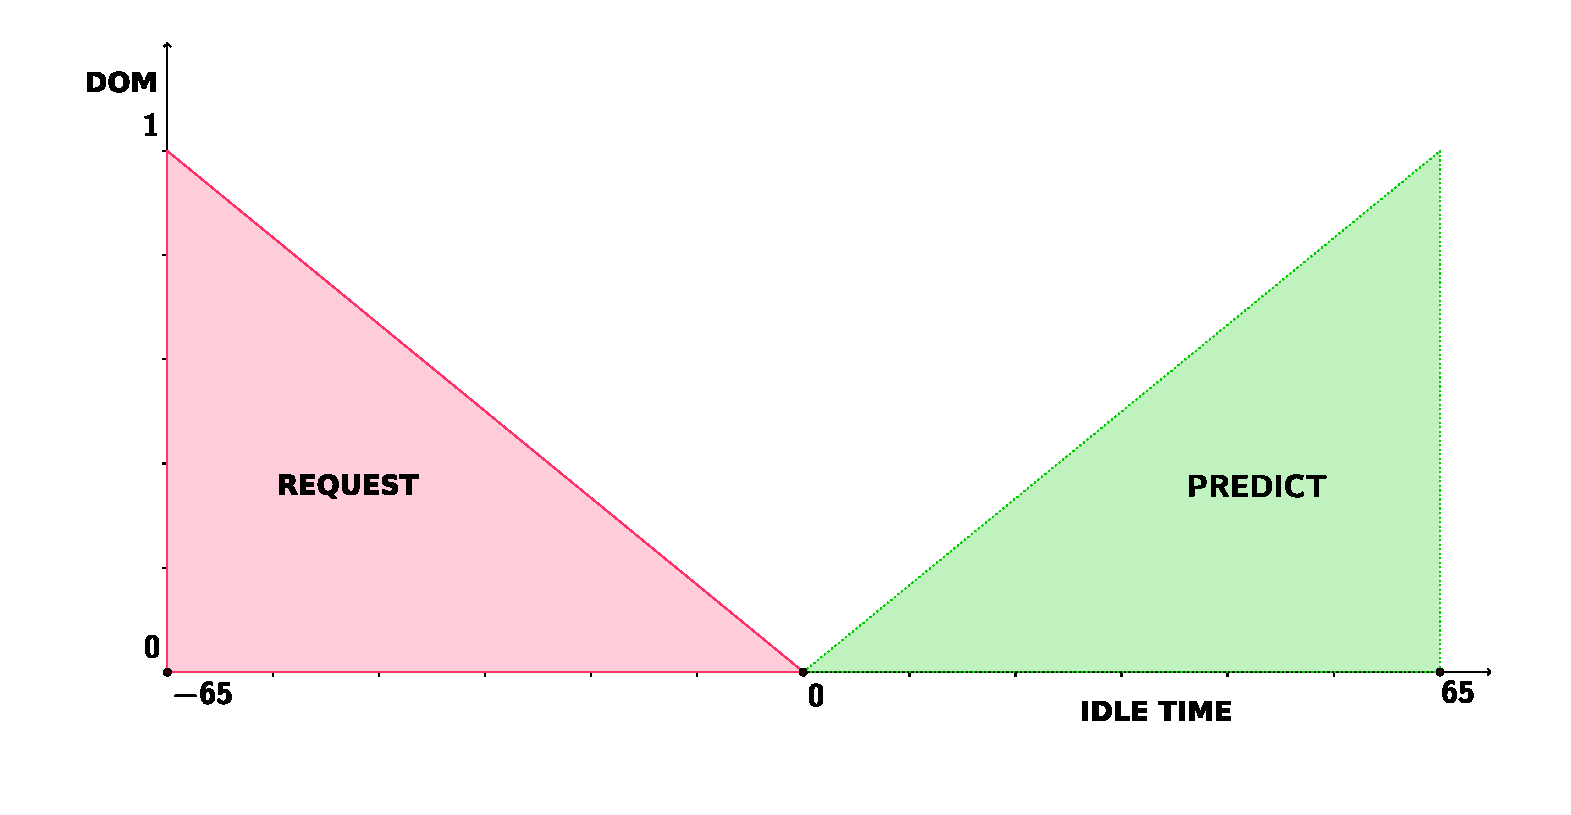
\includegraphics[scale=0.58]{4/figures/result_sets.pdf}
\caption{Idle Time Fuzzy Sets}
\label{idle_sets}
\end{figure}

When all input variables have been fuzzified and degrees of membership calculated, then the next step is to fire all predefined rules. For each sensor, there is a collection of 3 rules, making a total of 9 rules (here $x \in \{hall, temp, light\}$):

\begin{enumerate}
\item IF $x$ IS $x\_changed\_left$ OR $x\_changed\_right$ AND $x\_predictability$ IS $not\_predictable$ OR $predictable$ THEN $request$
\item IF $x$ IS $x\_same$ AND $x\_predictability$ IS $not\_predictable$ THEN $request$
\item IF $x$ IS $x\_same$ AND $x\_predictability$ IS $predictable$ THEN $predict$
\end{enumerate}

The previously calculated degrees of membership are fed into these rules. For $AND$ relationship, the minimum value is selected, for $OR$ relationship, the maximum value is selected. For each rule, the output variable received a DOM equal to the DOM of the premise. When all rules have been evaluated, the results are defuzzified into a single crisp value, which is the idle time decision. This process is called defuzzification.

During defuzzification the DOMs of result sets $request$ and $predict$ for each rule are combined into a single DOM for the specified set. For this, $request$ output has an $OR$ relationship (maximum value) and the $predict$ set has an $AND$ relationship (minimum value). These relationships mean that the most inaccurate sensors would be represented in the final result. For example if $hall$ has a DOM of 1.0 to $predict$, but $temp$ has a DOM of 0.5 to $predict$, then the outcome would be a DOM of 0.5, because we need the output for least accurate sensors. For $request$ this logic is reversed as the maximum DOM to $request$ represents the output for the least accurate sensor. 

The next step is to get the crisp result value. For this process, the idle time values for $predict$ and $request$ set membership functions at the specified DOM are calculated. $x$ is found the equation $f(x) = DOM$, where $x$ is the idle time and $f$ is the membership function. $request$ and $predict$ membership functions are symmetric with the axis being in the point $x = 0$ as seen in \autoref{idle_sets}. The final defuzzified idle time is equal to $max\{x_{predict} - x_{request}, 10\}$. Meaning that if the DOM to $request$ was higher that to predict, then the default idle time of 10 seconds is returned. Otherwise the value at the center point of the two results is returned.

When the crisp result is received from the fuzzy control system and idle time is longer than 10 seconds, future data is predicted for the idle period. This means that using the regression models, future values with 10 second intervals are inserted into the database for each sensor. 

Finally, the idle time with a minimum value of 10 seconds is written as a JSON format string to the response body of the HTTP request. A sample response would look like:\\ \todo{add a sample response here}

\begin{lstlisting}
HTTP/1.1 200 OK
Content-Type: application/json;charset=utf-8
Content-Length: 12
Connection: close
Server: Jetty(7.2.0.v20101020)

{"idle": 34}
\end{lstlisting}

\section{Results}

\begin{figure}[h!]
\centering
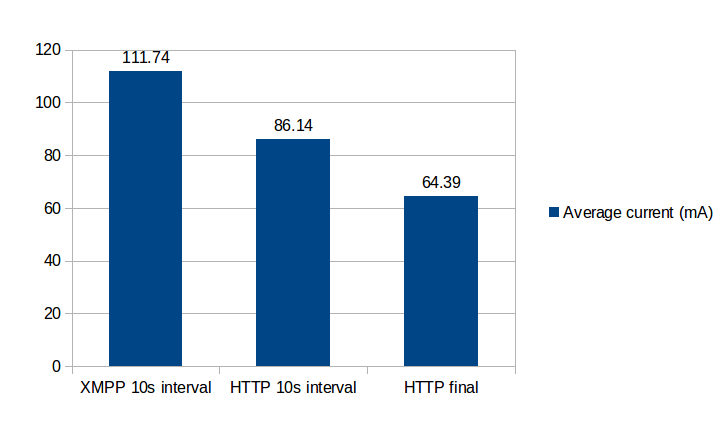
\includegraphics[scale=1]{4/figures/final_measurements.png}
\caption{Final Measurements Comparison}
\label{final_measurements}
\end{figure}

\begin{table}[h]
\centering
  \begin{tabular}{|l|l|l|l|}
    \hline
     & Average current (mA) & Percentage & Improvement \\ \hline
    XMPP 10s interval & 111.74 & 100\% & \\ \hline
    HTTP 10s interval & 86.14 & 77\% & 23\% \\ \hline
    HTTP final & 64.39 & 58\% & 42\% \\
    \hline
  \end{tabular}
\caption{Overview of Final Results}
\label{table}
\end{table}

\todo{Describe tests carried out}\\
\todo{Make a test with a 9V battery}\\
\todo{Graphs with improved power consumption figures on it, description of what changed and how/why}
\todo{Graph with 10s idle time as the worst-case scenario here}

% ---------------------------------------------------------------------------
%: ----------------------- end of thesis sub-document ------------------------
% ---------------------------------------------------------------------------

		% how the solution solved the problem - your solution
%\include{4/casestudies}			% functional scenario
% this file is called up by thesis.tex
% content in this file will be fed into the main document

%: ----------------------- name of chapter  -------------------------
\chapter{Conclusions} % top level followed by section, subsection

Pervasive applications have become more common in recent years and therefore mobile applications need to take advantage of the possibilities they offer. To provide this contextual information, a prototype solution was developed, which registers sensor data from an Arduino-based module and saves it in a data server.

The prototype solution was further developed in this thesis to increase battery performance and therefore the usability of the prototype. For this, a variable sensor reading interval solution was developed, which consists of a fuzzy control engine and simple linear regression model. Moreover, the sensor module was improved to enable sleep mode during periods of inactivity to fully utilize the variable sensor reading times.

A switch from XMPP to HTTP was made on the communication protocol part. This switch was necessary to enable sleep mode in the sensor modules, since XMPP session negotiation is a verbose process and therefore takes longer than making a simple HTTP request. The move to HTTP decreased connection initialization and data sending times, which enabled the module to utilize sleep mode for longer periods.

Several tests were carried out to measure the actual benefits of the proposed improvements and the results were positive. Two tests, with improvements of 80\% and 111\% over the previous prototype's battery lifetime, were carried out. These tests show that the proposed solution of enabling sleep mode in the sensor module for idle periods decreases power consumption and enables the module to perform its tasks for a longer period of time.
 
%: ----------------------- paths to graphics ------------------------

% change according to folder and file names
\ifpdf
    \graphicspath{{X/figures/PNG/}{X/figures/PDF/}{X/figures/}}
\else
    \graphicspath{{X/figures/EPS/}{X/figures/}}
\fi

%: ----------------------- contents from here ------------------------

% ---------------------------------------------------------------------------
%: ----------------------- end of thesis sub-document ------------------------
% ---------------------------------------------------------------------------

			% final conclusions

% this file is called up by thesis.tex
% content in this file will be fed into the main document

\chapter{Related Work} % top level followed by section, subsection

A solution for energy-efficient data collection for clustering-based wireless sensor networks has been suggested \cite{cluster_wsn_paper}. This solution has wireless sensor clusters with a head node, which actively decides if new sensor data should be requested from the nodes or if they can be predicted. The communication with the central data collection point goes through cluster heads only, which reduces transfer overhead. This is similar to the current thesis in a sense that data is predicted or requested and then forwarded, with the exception that this prototype does not have clusters and extra complexity that comes with clustering. 
The general implementation idea has been taken from this solution and prediction algorithm details, because in both cases simple linear regression is used to predict sensor data. \todo{improve this?}

\todo{check linear regression reference from that thesis}

The previous prototype \cite{prev_thesis} is the main basis of this work as it was the starting point. The previous implementation used XMPP as the communication protocol and a fixed interval data collection. XMPP has several advantages over simple HTTP requests, mainly because the protocol supports message queues and security. However, actually useful security options \todo{which was it?}(SSL/TLS) are unavailable due to their overhead and implementation complexity for Arduino boards. On the other hand, XMPP protocol has communication overhead which reduces its usability when fast connection establishment and data transmission is required.

A similar system of Arduino sensor module and a central data collection server was discussed in three blog posts \cite{arduino_blog_1,arduino_blog_2,arduino_blog_3}. The posts focused on power consumption of Arduino boards, because similarly a 9V battery could not power the device long enough. The main focus point the the posts was hardware modifications to the boards by either using a more power-efficient Arduino board, \todo{maybe reference arduino mini here?} replacing certain components of the board or making their own hardware using a breadboard. On the software side, a similar sleep and wake cycle solution was developed. The sleep and wake cycles were implemented using the internal watchdog timer similar to what is used in the JeeLib library's Port class \cite{jeelib_port}.



% ----------------------- paths to graphics ------------------------

% change according to folder and file names
\ifpdf
    \graphicspath{{8/figures/PNG/}{8/figures/PDF/}{8/figures/}}
\else
    \graphicspath{{8/figures/EPS/}{8/figures/}}
\fi

% ----------------------- contents from here ------------------------




% ---------------------------------------------------------------------------
%: ----------------------- end of thesis sub-document ------------------------
% ---------------------------------------------------------------------------



 






	                % related work

% this file is called up by thesis.tex
% content in this file will be fed into the main document

\chapter{Future Research Directions} % top level followed by section, subsection

The changes made in this thesis are done with the notion of improving on a proof of concept prototype. This means that the changes are done to prove a concept as well. 
Hence, several aspects of the changes implemented can be improved upon.

Firstly, starting with the Arduino sensor module, the hardware side of the module can greatly affect the power consumption of the device. Currently, Arduino Mega ADK is used, which is one of the most power-hungry boards available. Currently, the board on average draws 55$mA$ in sleep mode, which is very close to the average current drawn as seen in \autoref{final_measurements}. When this number is lowered, the average current drawn will decrease and thus improve battery lifetime. 

Secondly, the server-side client's fuzzy control engine and prediction models can be improved. At the moment, the fuzzy control engine checks if the measured value has changed from a previous measurement by a degree $x$. If it has, a new measurement is requested. However, this configuration does not cover the case when the measurement values changes steadily by a degree which is larger than the acceptable $measure\_error$. In this case, the changes in value might be large, but if they are steady, then the future values could still be predictable. 

Finally, the prediction model can be improved upon to better handle extreme values, because currently, a large enough deviation can cause the model to become inaccurate. The selected $measure\_error$ and $regressin\_error$ values can be adjusted to better suit the selected sensors and their data ranges. At the moment, the values are based on a trial and error tuning of the models to suit the needs of the prototype level device. However, in an actual implementation environment, these values should be based of the type of information needed from the sensors. For example, a small change in the light sensor measurements might indicate that an object (a bird) has flown past the sensor, but if the goal is to measure the cloudiness of the sky or the time of day, the acceptable deviations in the sensor values can be larger to ignore small fluctuations.  

















% ----------------------- paths to graphics ------------------------

% change according to folder and file names
\ifpdf
    \graphicspath{{8/figures/PNG/}{8/figures/PDF/}{8/figures/}}
\else
    \graphicspath{{8/figures/EPS/}{8/figures/}}
\fi

% ----------------------- contents from here ------------------------
% ---------------------------------------------------------------------------
%: ----------------------- end of thesis sub-document ------------------------
% ---------------------------------------------------------------------------










		% future research directions

\backmatter
% this file is called up by thesis.tex
% content in this file will be fed into the main document
\chapter[Resümee]{Mobiilsetele kasutajatele sensoritelt kogutud keskonnapõhiste andmete energiateadlik edastamine} % top level followed by section, subsection
\textbf{Bakalaureusetöö (6 EAP)}\\
\textbf{Lauris Kruusamäe}\\

Tänapäeval levib järjest rohkem rakendusi, mis tajuvad ümbritsevat keskkonda ning pakuvad sellele põhinevalt kasutajale lisavõimalusi. Selliste võimaluste pakkumiseks on arendatud prototüüp, mis kogub keskkonna kohta andmeid kasutades Arduino platvormil põhinevad sensorite moodulit ning keskset andmet kogumise serverit. 

Käesolevas töös arendati antud prototüüpi edasi, et tõsta aku vastupidavust ning seeläbi parandada lahenduse kasutatavust. Selleks loodi varieeruva sensoriandmete saatmise intervalliga lahendus, mis koosneb hägusloogikat kasutavast kontrollsüsteemist ning lihtsa lineaarse regressiooni mudelist. Lisaks loodi lahendus, mis lubab sensorite moodulil vabadel hetkedel minna puhkerežiimi.

Töö käigus asendati seni kasutuselolev XMPP protokoll HTTP protokolli vastu, et parandada ühenduse loomise ajakulu ning lubada sensorite moodulil kauem puhkerežiimis olla.

Parandatud lahenduse tulemusi mõõdeti mitme testi käigus. Kaks põhilist testi, mille käigus sensorite moodul sai voolu 9-voldiselt patareilt, andsid vastavalt tulemusteks 80 ja 110 \% pikema eluea. Sellest tulenevalt saab eeldada, et pakutud puhkerežiimi ja muutuva intervalliga andmete kogumist kasutav lahendus parandab aku vastupidavust ning seega ka prototüübi kasulikkust.



% ----------------------- paths to graphics ------------------------

% change according to folder and file names
\ifpdf
    \graphicspath{{7/figures/PNG/}{7/figures/PDF/}{7/figures/}}
\else
    \graphicspath{{7/figures/EPS/}{7/figures/}}
\fi


% ----------------------- contents from here ------------------------






% ---------------------------------------------------------------------------
% ----------------------- end of thesis sub-document ------------------------
% ---------------------------------------------------------------------------
               % discussion of results

\newpage
% ----- LICENCE -------

\chapter{Licence}

\textbf{Non-exclusive licence to reproduce thesis and make thesis public}\\

I, Lauris Kruusamäe (date of birth: 30/12/1989), herewith grant the University of Tartu a free permit (non-exclusive licence) to: 

1.1. reproduce, for the purpose of preservation and making available to the public, including for addition to the DSpace digital archives until expiry of the term of validity of the copyright, and

1.2. make available to the public via the web environment of the University of Tartu, including via the DSpace digital archives until expiry of the term of validity of the copyright,

\begin{center}
Energy-aware Sensor Data Collection for Mobile Users\\
supervised by Huber Flores and Satish Narayana Srirama,
\end{center}

2. I am aware of the fact that the author retains these rights.

3. I certify that granting the non-exclusive licence does not infringe the intellectual property rights or rights arising from the Personal Data Protection Act. 

\begin{center}
\vspace{3cm}
Tartu, 13.05.2013
\end{center}
\newpage

% --------------------------------------------------------------
%:                  BACK MATTER: appendices, refs,..
% --------------------------------------------------------------

% the back matter: appendix and references close the thesis

%: ----------------------- bibliography ------------------------

% The section below defines how references are listed and formatted
% The default below is 2 columns, small font, complete author names.
% Entries are also linked back to the page number in the text and to external URL if provided in the BibTex file.

% PhDbiblio-url2 = names small caps, title bold & hyperlinked, link to page 
%\begin{multicols}{2} % \begin{multicols}{ # columns}[ header text][ space]
\begin{small}
 % tiny(5) < scriptsize(7) < footnotesize(8) < small (9)

%\bibliographystyle{Latex/Classes/PhDbiblio-url2} % Title is link if provided
%\renewcommand{\bibname}{References} % changes the header; default: Bibliography

%\bibliography{9_backmatter/references} % adjust this to fit your BibTex file


\bibliographystyle{elsarticle-num}	% references style
\bibliography{thesis}
			% references bibtex file  - utilize JabRef
\end{small}

% --------------------------------------------------------------
% Various bibliography styles exit. Replace above style as desired.

% in-text refs: (1) (1; 2)
% ref list: alphabetical; author(s) in small caps; initials last name; page(s)
%\bibliographystyle{Latex/Classes/PhDbiblio-case} % title forced lower case
%\bibliographystyle{Latex/Classes/PhDbiblio-bold} % title as in bibtex but bold
%\bibliographystyle{Latex/Classes/PhDbiblio-url} % bold + www link if provided

%\bibliographystyle{Latex/Classes/jmb} % calls style file jmb.bst
% in-text refs: author (year) without brackets
% ref list: alphabetical; author(s) in normal font; last name, initials; page(s)

%\bibliographystyle{plainnat} % calls style file plainnat.bst
% in-text refs: author (year) without brackets
% (this works with package natbib)
\chapter{Appendix A}

The Arduino sensor module sketch and server-side client implementation code can be accessed from https://github.com/huberflores/ArduinoXMPP/. The $master$ branch contains the original prototype \cite{prev_thesis}. The improved implementation is in the $dev$ branch, last change commit hash - $c5126a9a36dd362596444dbadc901ea083bf4031$.

The code, collected data and thesis $\LaTeX$ files are also available on a CD attached to the thesis.

% --------------------------------------------------------------

% according to Dresden med fac summary has to be at the end
%
% Thesis Abstract -----------------------------------------------------


%\begin{abstractslong}    %uncommenting this line, gives a different abstract heading
\begin{abstracts}        %this creates the heading for the abstract page

Nowadays, mobile applications are becoming more context aware due to technological
achievements which enable the applications to anticipate users’ intentions. This is
achieved through using the device’s own micromechanical artifacts that can be used to
perceive the environment. However, this is constrained to the hardware limitations of
devices as not all devices provide the same options. Moreover, perceiving the environment strains the battery and therefore has its impact on devices' everyday usage.

To remedy this, a proposed solution has been made in the thesis “Context Sensor Data on
Demand for Mobile Users Supported by XMPP” by Kaarel Hanson. The solution is to gather the environmental data by specialized sensor modules and store it in a data server. Afterwards, devices can query the data from the server and thus gain access to information beyond the capabilities of their own hardware.

The solution uses XMPP for transporting sensor data from Arduino microcontrollers (sensor modules) to the cloud. Arduino provides low-cost hardware, while the cloud offers the reliable and high-
availability means for storing and processing sensor data. However, the developed prototype shows that running on a 9V battery the microcontroller lasts for 101
minutes when using an Ethernet module for communications, and 161,5 minutes with a
WiFi module. These results are not good enough for remote data collection with limited access as the maintenance cost would be too high when the batteries need to be replaced frequently. 

This thesis proposes an optimisation for the system so that instead of reading and
sending sensor data every 10 seconds, the cloud server would notify the controller
when to start sending data and when to stop. This means implementing an algorithm
for detecting similar sensor data readings and notifying the microcontroller of needed
operations. With similar readings, the microcontroller could be put to an idle state for
limiting power consumption, which would prolong battery life.

The aim is to optimise the sensor reading process enough to prolong the Arduino
microcontroller’s battery life on a 9V battery.

\end{abstracts}
%\end{abstractlongs}


% ---------------------------------------------------------------------- 


%: Declaration of originality
%\include{9_backmatter/declaration}

\end{document}
